\section{第七章 \quad 对流传热的理论基础与计算}

\pt{对流传热定义}：流体流过固体壁面时发生的热量传递过程。特点：必须存在温差。流体与固体表面直接接触。是导热与流体宏观运动共同作用的结果。影响对流传热的因素：流动起因：强制对流、自然对流、混合对流。流动状态：层流、紊流，判据常用 $\mathrm{Re}=\rho ud/\mu$。换热表面几何因素：形状、尺度、相对位置、表面粗糙情况；也区分内流与外流。是否存在相变：沸腾、凝结等。流体物性：$\lambda$、$\rho$、$c_p$、$\mu$、$\gamma$ 等。

%{
% \centering
% 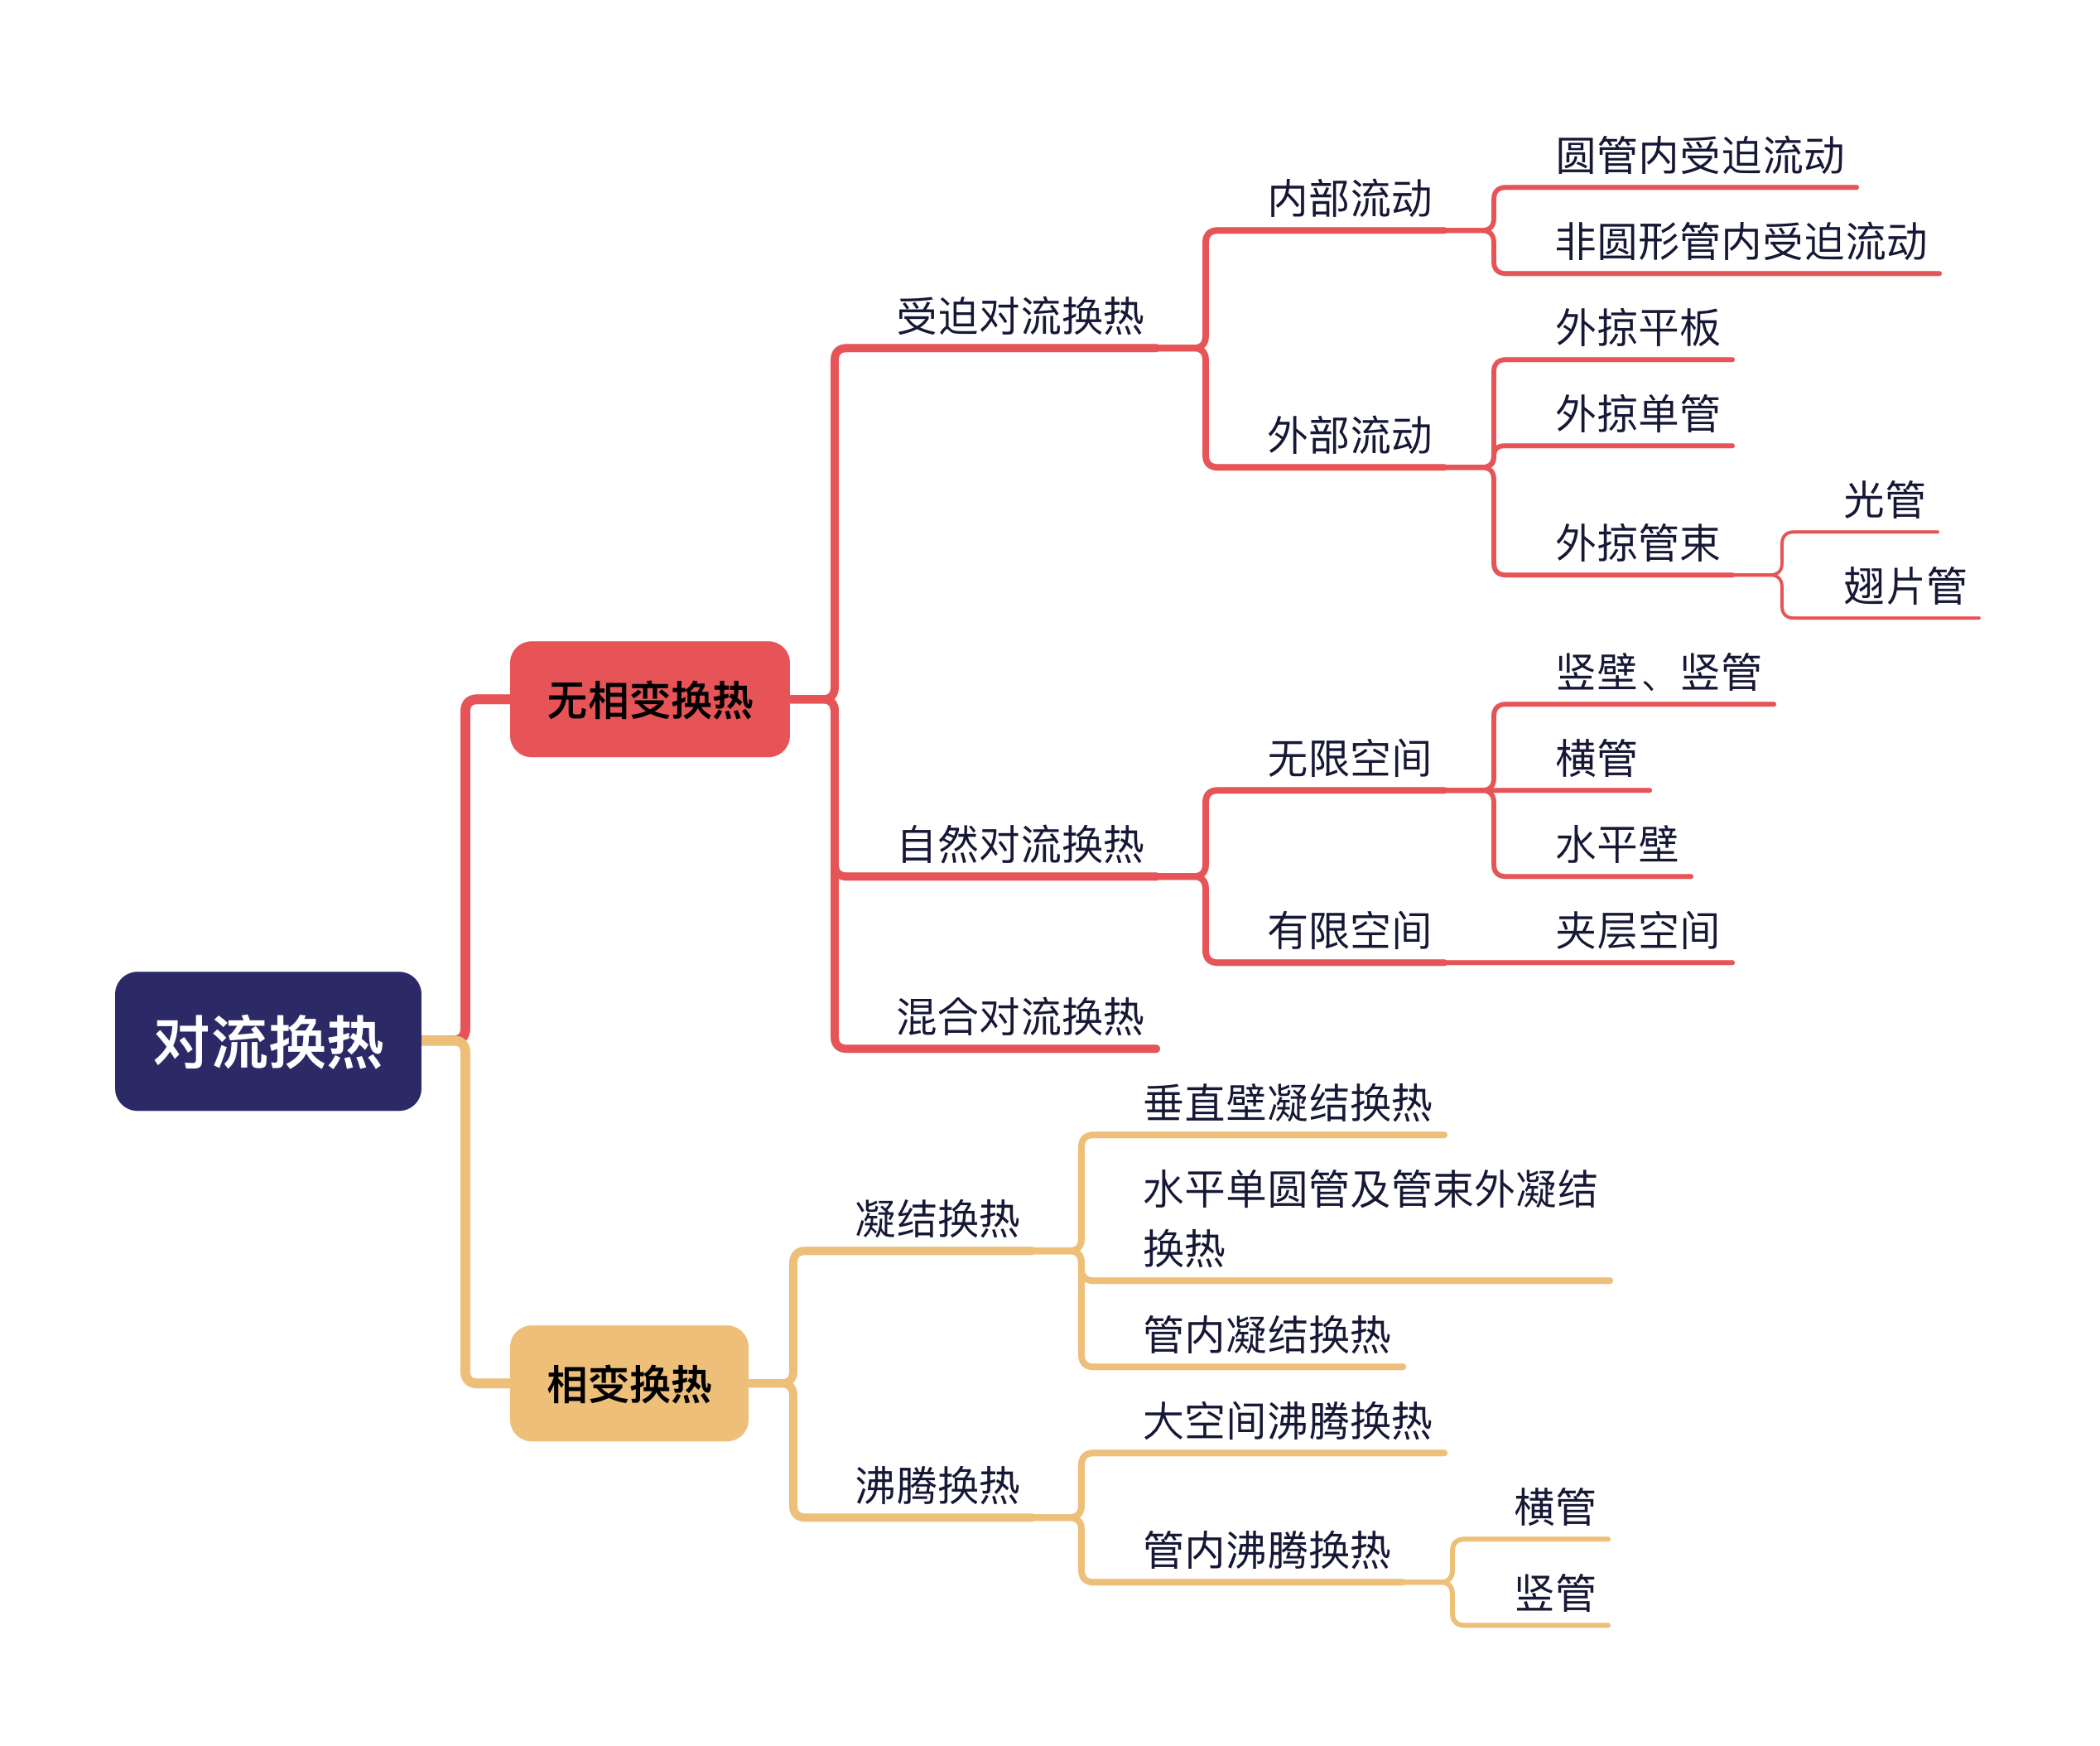
\includegraphics[width =.8\linewidth]{figures/7对流换热的分类.png}
%}

\pt{换热分类}：有无相变-流动起因-几何因素-流动状态\\
\pt{无相变换热}：受迫对流换热（内部流动：圆管、非圆形管；外部流动：外掠平板、外掠单管、外掠管束）；自然对流换热（无限空间：竖壁/竖管、横管、水平壁；有限空间：夹层空间）；混合对流换热。\\
\pt{相变换热}：凝结换热（垂直壁、水平单圆管及管束外、管内）；沸腾换热（大空间、管内）。

\pt{研究对流传热方法}分析法：采用数学分析求解，有指导意义。实验法：通过大量实验获得 $h$ 的计算式，是目前主要途径。比拟法：利用热量传递与动量传递的共性，建立 $h$ 与阻力系数之间关系，但限制较多。数值法：思想类似导热问题数值求解，发展迅速。

\pt{从温度场计算 $h$}：贴近壁面的薄层流体几乎不流动，热量传递主要靠导热。壁面局部热流密度：$q_{w,x}=-\lambda\left.\frac{\partial t}{\partial y}\right\vert_{y=0,x}$。换热热流密度：$q_{c,x}=h_x(t_{w,x}-t_{\infty})$。$q_{w,x}=q_{c,x}$，$h_x=-\lambda\frac{\left.\partial t/\partial y\right\vert_{y=0,x}}{t_{w,x}-t_{\infty}}$。

与导热第三类边界条件区别：导热问题中 $h$ 已知；这里 $h$ 是待求量。导热问题中 $\lambda$ 是固体导热系数；这里 $\lambda$ 是流体导热系数。导热问题中 $t$ 是固体温度；这里 $t$ 是流体温度。

\divider

%\subsection{对流问题的数学描述}

\pt{对流问题求解思路}流场由连续方程、运动方程描述。温度场由能量方程描述。求得温度场后，再由壁面温度梯度求 $h_x$。
\pt{简化假设}:二维问题。不可压缩、牛顿流体。常物性、无内热源。流速不高，忽略黏性耗散。不计流体与壁面之间的辐射换热。


\pt{能量稳态方程}

$\underbrace{\rho c_p\frac{\partial t}{\partial\tau}}_{\text{非稳态项}}+\underbrace{\rho c_p(u\frac{\partial t}{\partial x}+\nu\frac{\partial t}{\partial y})}_{\text{对流项}}=\underbrace{\lambda(\frac{\partial^2t}{\partial x^2}+\frac{\partial^2t}{\partial y^2})}_{\text{导热项}}$

$u,v$ 分别为 $x,y$ 方向的速度分量

\pt{物理含义}：对流传热温度场来自能量守恒与“导热 + 对流”的热量输运形式。对流传热中的微元体是固定空间内的开口系统，有流体流入与流出。总能量关系可写成 $\Phi=\partial U/\partial \tau+H_{\mathrm{out}}-H_{\mathrm{in}}$。 导热项：单位时间内由导热导入微元体的净热量：$\Phi=\lambda(\partial^2 t/\partial x^2+\partial^2 t/\partial y^2)\mathrm{d}x\mathrm{d}y$。热力学能增量：$\partial U/\partial \tau=\rho c_p(\partial t/\partial \tau)\mathrm{d}x\mathrm{d}y$。焓差项：不可压缩流体下，$H_{\mathrm{out}}-H_{\mathrm{in}}=\rho c_p(u\partial t/\partial x+v\partial t/\partial y)\mathrm{d}x\mathrm{d}y$。

当 $u=v=0$ 时，方程退化为纯导热方程

\pt{控制方程}：

\pt{能量微分方程}$\rho c_{p}\left(\frac{\partial t}{\partial\tau}+u\frac{\partial t}{\partial x}+\nu\frac{\partial t}{\partial y}\right)=\lambda\left(\frac{\partial^{2}t}{\partial x^{2}}+\frac{\partial^{2}t}{\partial y^{2}}\right)$
\pt{连续性方程} $\frac{\partial u}{\partial x}+\frac{\partial\nu}{\partial y}=0$
\pt{运动微分方程}$\rho\frac{\mathrm{D}u}{\mathrm{\tau}}=\vec{F}-\nabla \vec{p}+\mu\nabla^2u$

%$$
%    \left\{
%    \begin{aligned}
%         & \frac{\partial u}{\partial x}+\frac{\partial\nu}{\partial y}=0 \\&\rho(\frac{\partial u}{\partial\tau}+u\frac{\partial u}{\partial x}+\nu\frac{\partial u}{\partial y})=F_{x}-\frac{\partial p}{\partial x}+\mu(\frac{\partial^{2}u}{\partial x^{2}}+\frac{\partial^{2}u}{\partial y^{2}})\\&\rho(\frac{\partial\nu}{\partial\tau}+u\frac{\partial\nu}{\partial x}+\nu\frac{\partial\nu}{\partial y})=F_{y}-\frac{\partial p}{\partial y}+\mu(\frac{\partial^{2}\nu}{\partial x^{2}}+\frac{\partial^{2}\nu}{\partial y^{2}})\\&\rho c_{p}\left(\frac{\partial t}{\partial\tau}+u\frac{\partial t}{\partial x}+\nu\frac{\partial t}{\partial y}\right)=\lambda\left(\frac{\partial^{2}t}{\partial x^{2}}+\frac{\partial^{2}t}{\partial y^{2}}\right)\\&h_{x}=-\frac{\lambda}{t_{w,x}-t_{\infty}}\left.\frac{\partial t}{\partial y}\right\vert_{y=0,x}
%    \end{aligned}
%    \right.
%$$

对二维、不可压、常物性、牛顿流体、无内热源问题，未知量为 $u$、$v$、$t$、$p$、$h_x$，无第三类边界条件，因为 $h_x$ 为未知量。方程非线性，运动方程与能量方程耦合，因此引入边界层概念来简化控制方程组。

\divider

%\subsection{边界层型对流传热问题的数学描述}

\pt{流动边界层}定义：流体流过固体壁面时，由于黏性作用，在壁面附近形成速度剧烈变化的薄层，称为流动边界层或速度边界层。速度边界层厚度：定义为速度达到主流速度 $99\%$ 的位置，即 $u_{\delta}=0.99u_{\infty}$。

\pt{流动边界层特点}：$\delta$ 比壁面尺度 $l$ 小一个数量级以上，$\delta\ll l$。边界层内也有层流和湍流之分；外掠平板临界雷诺数 $\mathrm{Re}_c=5\times 10^5$。边界层内沿厚度方向速度梯度很大，边界层外速度梯度近似为 $0$。$\delta$ 沿流动方向逐渐增加。因边界层很薄，可近似认为同一截面上边界层内压强等于外边界压强，即 $y$ 方向压强近似相等。边界层内黏性力与惯性力同一数量级。

\pt{引入速度边界层的意义}：流动区域可分为主流区和边界层区。主流区可近似看作理想流体流动。只在边界层区考虑黏性作用。

\pt{温度边界层}：对流传热时，壁面附近温度发生剧烈变化的薄层称为温度边界层或热边界层。

\pt{热边界层厚度}：可用 $(T-T_w)\vert_{\delta_t}=0.99(T_{\infty}-T_w)$ 表征。热边界层厚度 $\delta_t$ 也满足 $\delta_t\ll l$。

\pt{温度边界层意义}：温度场也可分为主流区和边界层区；主流区温度变化可看作近似为零；只需重点确定边界层区内流体温度分布。

\pt{层流与湍流热边界层}：湍流边界层贴壁处温度梯度明显大于层流。因 $h_x$ 与壁面温度梯度有关，湍流换热强于层流。

\pt{普朗特数}：$\mathrm{Pr}=\nu/a$。 $\nu$ 表征动量扩散能力，越大则黏性影响传递越远，流动边界层越厚。$a$ 表征热扩散能力，越大则温度扰动传递越快，热边界层越厚。$\delta/\delta_t\approx \mathrm{Pr}^{1/3}$，$\mathrm{Pr}>1$ ，$\delta>\delta_t$；$\mathrm{Pr}<1$ ，$\delta_t>\delta$。（通常）

流体按 $\mathrm{Pr}$ 分类：高普朗特数流体：如油类，约 $10^2\sim 10^3$。中等普朗特数流体：约 $0.7\sim 10$，如气体 $0.7\sim 1.0$，水 $0.9\sim 10$。低普朗特数流体：如液态金属，约 $0.01$。

简化后的二维、稳态边界层对流传热微分方程组：\\
\pt{连续方程}：$\frac{\partial u}{\partial x}+\frac{\partial\nu}{\partial y}=0$。\\
\pt{$x$ 方向动量方程}：$u\frac{\partial u}{\partial x}+\nu\frac{\partial u}{\partial y}=-\frac{1}{\rho}\frac{dp}{dx}+\upsilon\frac{\partial^{2}u}{\partial y^{2}}$。\\
\pt{能量方程}：$u\frac{\partial t}{\partial x}+\nu\frac{\partial t}{\partial y}=a\frac{\partial^{2}t}{\partial y^{2}}$。\\
\pt{局部换热系数}：$h_{x}=-\frac{\lambda}{t_{w,x}-t_{\infty}}\frac{\partial t}{\partial y}|_{y=0,x}$。\\
$y=0$，$u=0$，$v=0$，$t=t_w$；$y\to\infty$，$u=u_{\infty}$，$t=t_{\infty}$。

未知参数 $u.v.t.h_x$ 适用条件：二维、稳态、不可压缩常物性、牛顿流体、无内热源、重力场可忽略、主流方向二阶导数可忽略。若流场产生旋涡，如湍流，则需用完整控制方程组描述。

\divider

%\subsection{外掠等温平板对流传热的解}

恒定壁温时流体纵掠平板换热，且流态为层流。假设恒定壁温；流体纵向掠过平板；二维、稳态、无内热源、重力场可忽略；主流场匀速、匀温；对外掠等温平板，主流压强梯度为 $-\mathrm{d}p/\mathrm{d}x=0$。

\pt{解的形式}：局部换热系数 $h_x=0.332\frac{\lambda}{x}\left(\frac{u_\infty x}{\nu}\right)^{0.5}\left(\frac{\nu}{a}\right)^{1/3}=0.332\frac{\lambda}{x}\mathrm{Re}^{0.5}\mathrm{Pr}^{1/3}$，局部努塞尔数 $\mathrm{Nu}_x=0.332\mathrm{Re}_x^{0.5}\mathrm{Pr}^{1/3}$，局部雷诺数 $\mathrm{Re}_x=\frac{u_\infty x}{\nu}$，离平板前缘 $x$ 处边界层厚度 $\frac{\delta}{x}=\frac{5.0}{\sqrt{\mathrm{Re}_x}}$，$\delta = 5.0\sqrt{\frac{\nu x}{u_\infty}}$，范宁局部摩擦系数 $c_f =\frac{t_w}{0.5\rho {u_\infty}^2}=\frac{0.664}{\sqrt{\mathrm{Re}_x}}$，流动边界层与热边界层之比 $\delta/\delta_t\cong \mathrm{Pr}^{1/3}$，适用条件 $\mathrm{Re}<5\times 10^5$（以上所有公式）

$\mathrm{Nu}$ 数与 $\mathrm{Bi}$ 数的区别：局部努塞尔数：$\mathrm{Nu}_x=h_xx/\lambda$；毕渥数：$\mathrm{Bi}=hl/\lambda$；$\lambda$ 不同：$\mathrm{Nu}$ 中的 $\lambda$ 是流体导热系数；$\mathrm{Bi}$ 中的 $\lambda$ 是导热物体内部的导热系数；$h$ 的角色不同：$\mathrm{Nu}$ 中的 $h$ 通常是待求的对流换热系数；$\mathrm{Bi}$ 中的 $h$ 常作为已知边界换热条件；物理含义不同：$\mathrm{Nu}$ 表示壁面上流体的无量纲温度梯度；$\mathrm{Bi}$ 表示导热热阻与对流换热热阻的相对大小。

长度为 $l$ 的等温平板平均换热系数：$h_l=\frac{\int_{0}^{l} h_x \, \mathrm{d}x}{l}$；层流平均换热系数：$h_l=0.664(\frac{\lambda}{l})\mathrm{Re}_l^{0.5}\mathrm{Pr}^{1/3}$；平均努塞尔数：$\mathrm{Nu}_l=0.664\mathrm{Re}_l^{0.5}\mathrm{Pr}^{1/3}$；$\mathrm{Nu}$、$\mathrm{Re}$ 中的特征长度为平板长度 $l$；物性参数定性温度取边界层平均温度：$t_m=(t_\infty+t_w)/2$。

\pt{比拟理论概念}：利用两个物理现象控制方程的类似性，通过测定其中一种现象的规律，获得另一现象的基本关系。对湍流换热，利用湍流中动量传递与热量传递机理类似，借助较易测定的湍流阻力系数推求湍流换热系数或 $\mathrm{Nu}$ 数。雷诺比拟：通过建立 $\mathrm{Nu}$ 与湍流阻力系数 $c_f$ 的关系，由 $c_f$ 求湍流对流换热近似解 $\mathrm{Nu}_x=c_f\mathrm{Re}_x/2$。平板湍流边界层阻力系数实验式：$c_f=0.0592\mathrm{Re}_x^{-1/5}$，适用 $\mathrm{Re}_x\le 10^7$。推得：$\mathrm{Nu}_x=0.0296\mathrm{Re}_x^{4/5}$，这是雷诺比拟结果，成立前提为 $\mathrm{Pr}=1$。用于一般流体时写成：$\mathrm{Nu}_x=0.0296\mathrm{Re}_x^{4/5}\mathrm{Pr}^{1/3}$

长平板 $l>x_c$ 时的分段处理：$x<x_c$：层流区，$\mathrm{Nu}_x=0.332\mathrm{Re}_x^{1/2}\mathrm{Pr}^{1/3}$；$x>x_c$：湍流区，$\mathrm{Nu}_x=0.0296\mathrm{Re}_x^{4/5}\mathrm{Pr}^{1/3}$。积分后平均努塞尔数：$\mathrm{Nu}_m=[0.664\mathrm{Re}_c^{1/2}+0.037(\mathrm{Re}_l^{4/5}-\mathrm{Re}_c^{4/5})]\mathrm{Pr}^{1/3}$。

\divider

%\subsection{相似原理与量纲分析}

对流换热研究方法：分析法，比拟法，基于相似理论的实验方法，数值计算方法。
需要解决的 Problem：对流传热实验变量多，实验中应测哪些量，是否所有物理量都测；对流传热实验数据如何整理，整理成什么样的函数关系；对流传热实验结果如何推广，实物实验无法开展时怎么办。

相似原理的基本内容：相似原理研究相似物理现象之间的关系。相似的物理现象：两个同类物理现象，如果在相应时刻、相应地点上，与现象有关的物理量一一对应成比例，则称两现象彼此相似。同类现象：由相同形式和内容的微分方程式描述，包括控制方程和单值性条件方程。注意区分“相似”与“类比/比拟”。对稳态对流换热，相似意味着换热面几何形状、温度场、速度场、物性场等相似。对非稳态问题，还要求相应时刻各物理量空间分布相似。

相似现象的特性：只有同类现象才能谈相似；彼此相似的现象，其有关物理量场分别相似；此相似的现象，其同名特征数，也称准则数，必定相等：两个相似的对流传热现象，其 $\mathrm{Nu}$ 数必定相等。

圆管内单相强制对流换热问题：$h=f(u,d,\lambda,\mu,\rho,c_p)$。
量纲分析目标：把有量纲变量关系化为无量纲准则关系。
上述问题有 $n=7$ 个物理量，涉及 $r=4$ 个基本量纲：时间 $T$、长度 $L$、质量 $M$、温度 $\Theta$。
所以可得到 $n-r=3$ 个无量纲准则数。
选 $u$、$d$、$\lambda$、$\mu$ 为基本物理量，其余 $h$、$\rho$、$c_p$ 与基本物理量组成 $\pi$ 方程。
得到：
$\pi_1=hd/\lambda=\mathrm{Nu}$;
$\pi_2=\rho ud/\mu=ud/\nu=\mathrm{Re}$;
$\pi_3=\mu c_p/\lambda=\nu/a=\mathrm{Pr}$。
因而强制对流关系可写成：$\mathrm{Nu}=f(\mathrm{Re},\mathrm{Pr})$。
自然对流换热：$\mathrm{Nu}=f(\mathrm{Gr},\mathrm{Pr})$。
混合对流换热：$\mathrm{Nu}=f(\mathrm{Re},\mathrm{Gr},\mathrm{Pr})$。
对流传热实验中，只需测量无量纲准则数所包含的物理量。研究其关系

应用相似原理可以减少实验次数，并得到有一定通用性的结果。应以已定特征数为参数安排实验。常用整理形式为幂函数形式：$\mathrm{Nu}=C\mathrm{Re}^n$。$\mathrm{Nu}=C\mathrm{Re}^n\mathrm{Pr}^m$。$\mathrm{Nu}=C\mathrm{Gr}^n\mathrm{Pr}^m$。$C$、$n$、$m$ 由实验数据确定，可用作图法或最小二乘法。这类无量纲准则数间关系式称为准则方程、特征数方程或实验关联式。\pt{管内强制湍流、流体被加热}时可整理得 $\mathrm{Nu}=0.023\mathrm{Re}^{0.8}\mathrm{Pr}^{0.4}$。

\pt{实验关联式的推广条件}：
判别物理现象相似的条件：
同名已定特征数相等。
单值性条件相似。
单值性条件包括：初始条件、边界条件、几何条件、物理条件。
已定特征数：由所研究物理现象中已知量组成的特征数。
只要对流现象满足相似条件，实验关联式就可以推广。
实物实验无法开展时，可以由满足相似条件的模型实验代替。
不能严格满足完全相似时，至少应保证对现象起决定作用的关键特征数相等。
使用准则方程时必须明确适用范围。
特征长度、特征流速、定性温度的选取方式必须与建立准则方程时一致。

常见\pt{相似准则数及物理意义}：
努塞尔数：$\mathrm{Nu}=hl/\lambda$，表示流体壁面处法向无量纲过余温度梯度。
雷诺数：$\mathrm{Re}=ul/\nu$，表示惯性力与黏性力的相对大小。
普朗特数：$\mathrm{Pr}=\nu/a$，表示动量扩散能力与热量扩散能力的相对大小。
格拉晓夫数：$\mathrm{Gr}=g\alpha_V\Delta t l^3/\nu^2$，表示浮升力与黏性力的相对大小。

\divider

%\subsection{内部强制对流传热实验关系式}

\pt{管槽内强制流动与传热的特点}

外部流动中边界层一般不受限制；内部流动中边界层会受到另一侧固体壁面的限制，可能发生边界层干扰或汇合。

\pt{管内流态判别}：层流临界雷诺数 $\mathrm{Re}_c=2300$；$2300<\mathrm{Re}<10000$ 为过渡区；$\mathrm{Re}>10000$ 为旺盛湍流区。管内存在入口段，边界层由零开始发展并最终汇合，入口段内传热强度由高逐渐减弱。

入口段长度估算：层流 $\ell_e/d\approx0.05\mathrm{Re}\mathrm{Pr}$；湍流 $\ell_e/d\approx60$。管内换热边界条件主要有两类：恒定热流密度、恒定壁温。特征速度一般取截面平均流速，课件给出 $u_m=\frac{\int_{A_c}\rho u,\mathrm{d}A}{\rho A_c}$。定性温度多取截面上流体平均温度，$t_f=\frac{\int_{A_c}c_p\rho tu\,\mathrm{d}A}{\int_{A_c}c_p\rho u\,\mathrm{d}A}$；工程中常取进出口截面平均温度 $t_f=(t'_f+t''_f)/2$。

牛顿冷却公式：$\Phi=hA\Delta t_m$。恒热流时，平均温差可取 $\Delta t_m=t_w-t_f$。恒壁温时，局部温差沿管长变化，应按热平衡式 $hA\Delta t_m=q_m c_p(t''_f-t'_f)$，并用对数平均温差 $\Delta t_m=\frac{t''_f-t'_f}{\ln((t_w-t'_f)/(t_w-t''_f))}$。

\pt{管内湍流 Dittus-Boelter 公式} $\mathrm{Nu}_f=0.023\mathrm{Re}_f^{0.8}\mathrm{Pr}_f^n$；流体被加热时 $n=0.4$，被冷却时 $n=0.3$。适用范围：$\mathrm{Re}=10^4\sim1.2\times10^5$，$\mathrm{Pr}=0.7\sim120$，$\ell/d\ge60$，光滑管湍流充分发展段。
中等温差限制：气体 $\Delta t\le50^\circ\mathrm{C}$，水 $\Delta t\le20\sim30^\circ\mathrm{C}$，油 $\Delta t\le10^\circ\mathrm{C}$；这里 $\Delta t=t_w-t_f$，不是进出口温差。
不适用于液态金属，因为液态金属 $\mathrm{Pr}\sim10^{-2}$。
入口段修正：若 $\ell/d<60$，引入 $c_l=1+(d/\ell)^{0.7}$。
弯管或螺旋管修正：二次流会破坏热边界层、强化传热；课件给出气体 $c_r=1+1.77d/R$，液体 $c_r=1+10.3(d/R)^3$。
大温差修正：气体被加热 $c_t=(T_f/T_w)^{0.5}$，气体被冷却 $c_t=1$；液体被加热 $c_t=(\mu_f/\mu_w)^{0.11}$，液体被冷却 $c_t=(\mu_f/\mu_w)^{0.25}$。
修正后公式为 $\mathrm{Nu}_f=0.023\mathrm{Re}_f^{0.8}\mathrm{Pr}_f^n c_t c_l c_r$。

\pt{管内湍流的 Gnielinski 公式}  \\ $\mathrm{Nu}_f=\frac{(f/8)(\mathrm{Re}_f-1000)\mathrm{Pr}_f}{1+12.7(f/8)^{1/2}(\mathrm{Pr}_f^{2/3}-1)}[1+(d/\ell)^{2/3}]c_t$。
Darcy 阻力系数为 $f=(1.82\lg\mathrm{Re}-1.64)^{-2}$。
适用范围：光滑管道湍流过渡区与充分发展段，$\mathrm{Re}=10^4\sim1.2\times10^5$，$\mathrm{Pr}=0.7\sim120$，$\ell/d\ge60$
物性修正：气体 $c_t=(T_f/T_w)^{0.45}$，且 $T_f/T_w=0.5\sim1.5$；液体 $c_t=(\mathrm{Pr}_f/\mathrm{Pr}_w)^{0.11}$，且 $\mathrm{Pr}_f/\mathrm{Pr}_w=0.05\sim20$。

D-B 公式形式简单；Gnielinski 公式精度更高，要求较高时优先使用


\pt{管内层流的 Sieder-Tate 公式}

管内层流充分发展换热中，热边界条件影响显著；充分发展段的 $\mathrm{Nu}$ 与 $\mathrm{Re}$ 无关。
工程换热设备中，层流常处于入口段范围，因此使用 Sieder-Tate 公式：$\mathrm{Nu}_f=1.86(\frac{\mathrm{Re}_f\mathrm{Pr}_f}{\ell/d})^{1/3}(\frac{\mu_f}{\mu_w})^{0.14}$。
适用条件：$\mathrm{Re}<2300$，均匀壁温，入口段层流，且温差影响已修正。$\mu_f/\mu_w=0.0044\sim9.75$，$\mathrm{Pr}_f=0.48\sim16700$， $\left(\frac{\mathbf{Re}_f\mathbf{Pr}_f}{l/d}\right)^{1/3}\left(\frac{\mu_f}{\mu_w}\right)^{0.14}\geq2$

\divider

%\subsection{外部强制对流传热实验关联式}

\pt{外掠等温平板}：层流 $\mathrm{Nu}_x=0.332\mathrm{Re}_x^{1/2}\mathrm{Pr}^{1/3}$，湍流 $\mathrm{Nu}_x=0.0296\mathrm{Re}_x^{4/5}\mathrm{Pr}^{1/3}$。平板计算注意：局部特征尺度取 $x$，平均换热时取板长 $\ell$；定性温度取 $t_m=(t_\infty+t_w)/2$；特征速度取来流速度 $u_\infty$。

\pt{横掠单管平均换热关联式}采用分段幂次式 $\mathrm{Nu}=C\mathrm{Re}^n\mathrm{Pr}^{1/3}$。
横掠单管三大特征量：定性温度 $t_f=(t_w+t_\infty)/2$；特征长度为管外径 $d$；特征速度为来流速度 $u_\infty$。
横掠单管适用范围：气体和液体均适用；$t_\infty=15.5\sim980^\circ\mathrm{C}$，$t_w=21\sim1046^\circ\mathrm{C}$，$\mathrm{Re}=0.4\sim4\times10^5$；计算时需按 $\mathrm{Re}$ 分段取 $C,n$。

\pt{纵掠单管}可视作长 $\ell$、宽 $\pi d$ 的外掠平板处理；层流和湍流仍可套用外掠平板局部关联式。$\mathrm{Nu}_x=0.332\mathrm{Re}_x^{1/2}\cdot \mathrm{Pr}^{1/3}$，$\mathrm{Re}<5\times10^5$，层流；$\mathrm{Nu}_x=0.0296\mathrm{Re}_x^{4/5}\mathrm{Pr}^{1/3}$

\pt{外掠球体}关联式为 $\mathrm{Nu}=2+(0.4\mathrm{Re}^{1/2}+0.06\mathrm{Re}^{2/3})\mathrm{Pr}^{0.4}(\mu_\infty/\mu_w)^{1/4}$。定性温度取来流温度，特征速度取来流速度，特征长度取球直径；适用范围为 $\mathrm{Pr}=0.71\sim380$，$\mathrm{Re}=3.5\sim7.6\times10^6$。

\pt{横掠管束}中，管间相互影响明显；叉排扰动强、换热强、阻力大；顺排扰动小、换热弱、阻力小且易清洗。
管束后排会受前排影响，冲刷方向也会影响换热。
\pt{茹卡乌斯卡斯公式 Zhukauskas}写作 $\mathrm{Nu}_f=C\mathrm{Re}_{f,\max}^m\mathrm{Pr}_f^n(\mathrm{Pr}_f/\mathrm{Pr}_w)^k(s_1/s_2)^p\varepsilon_n$。
管束计算中，定性温度取进出口流体平均温度 $t_f=(t'_f+t''_f)/2$，特征长度取管外径 $d$，特征速度取最窄截面平均流速。
适用条件：管排总数 $\ge16$；小于 16 时要修正；管距参数 $s_1,s_2$ 已含在公式中；适用 $\mathrm{Pr}=0.6\sim500$，$\mathrm{Re}=1\sim2\times10^6$。

\divider

%\section{自然对流实验关联式}

自然对流传热是由温度场不均匀引起密度不均匀，并在重力作用下产生浮升力而形成的流动与传热现象。
自然对流的流动与传热不可分割；它不依靠泵或风机等外力推动。
不均匀温度场不一定引起自然对流：若热流体在上、冷流体在下，可能形成稳定分层；若热流体在下、冷流体在上，则更容易形成不稳定环流。
自然对流通常传热较弱，常成为主要热阻，但优点是经济、安全、安静。
自然对流总换热量常需同时考虑与周围气体的自然对流和与周围表面的辐射传热，二者量级可能相当。
热竖壁自然对流边界层中，壁面处 $y\to0$ 有 $u=0,T=T_w$；远离壁面 $y\to\infty$ 有 $u=0,T=T_\infty$；速度在边界层内部有最大值。
自然对流也分层流和湍流；层流时局部表面传热系数随高度增加而减小，过渡时增加，旺盛湍流时局部表面传热系数近似为常量。
自然对流流态判别主要用\pt{格拉晓夫数} $\mathrm{Gr}$。
自然对流按空间分为大空间和有限空间；大空间指边界层在发展过程中不受干扰，有限空间指空间大小会影响传热效果。
课件给出大空间判据示意：若 $a/H>0.28$、$b/H>0.01$，可按大空间处理。

\pt{自然对流控制方程与特征数}

局部表面传热系数可由壁面温度梯度写作 $h_x=-\frac{\lambda}{t_{w,x}-t_\infty}(\frac{\partial t}{\partial y})\vert_{y=0,x}$。
对竖直平板上空气被加热的边界层，可忽略 $x$ 方向二阶导数项和 $y$ 方向动量方程，得到边界层型方程。
浮升力来源可写作 $\frac{g}{\rho}(\rho_\infty-\rho)=g\alpha_V\theta$，即由“温压”驱动。
格拉晓夫数为 $\mathrm{Gr}=\frac{g\alpha_V\Delta t l^3}{\nu^2}$，表示浮升力与黏性力之比。
自然对流中，能量方程还引入 $\mathrm{Pr}$，因此 $\mathrm{Nu}=f(\mathrm{Gr},\mathrm{Pr})$。
瑞利数为 $\mathrm{Ra}=\mathrm{Gr}\mathrm{Pr}$，常将自然对流关联式写成 $\mathrm{Nu}=C(\mathrm{Gr}\mathrm{Pr})^n=C\mathrm{Ra}^n$。

\pt{大空间自然对流}

大空间自然对流平均努塞尔数关联式：$\mathrm{Nu}=C(\mathrm{Gr}\mathrm{Pr})^n=C\mathrm{Ra}^n$。
特征温度取边界层平均温度 $t_m=(t_w+t_\infty)/2$。
特征长度：竖平板和竖圆柱取表面高度 $l$，横圆柱取外径 $d$。
非均匀壁温情形也可近似套用均匀壁温关联式，取平均壁温计算。
气体的体膨胀系数可按理想气体取 $\alpha_V=1/T$，液体的 $\alpha_V$ 需查物性手册。
一般层流时 $n=1/4$，湍流时 $n=1/3$。
课件例题 1 比较 $l/d=10$ 的金属柱体水平或垂直放置冷却：在两种情形均为层流且忽略端面散热时，计算得 $h_l/h_d=0.69$，所以从自然对流冷却角度看，水平放置散热更强。

\pt{有限空间对流}

典型有限空间包括竖封闭夹层和水平封闭夹层。
有限空间中，夹层厚度 $\delta$ 对流动开展有重要影响；冷热壁面温差是流动动力。
有限空间常用 $\delta$ 作为特征长度，取 $\mathrm{Nu}_\delta=h\delta/\lambda$，$\mathrm{Gr}_\delta=\frac{g\alpha_V\delta^3(t_{w1}-t_{w2})}{\nu^2}$，$t_m=(t_{w1}+t_{w2})/2$。
当 $\mathrm{Gr}_\delta$ 很小时，封闭空气夹层近似为纯导热：竖夹层 $\mathrm{Gr}_\delta\le2860$，水平夹层 $\mathrm{Gr}_\delta\le2430$。
封闭空气夹层总传热量等于自然对流换热和辐射换热之和。
竖封闭夹层关联式为 $\mathrm{Nu}_\delta=C(\mathrm{Gr}_\delta\mathrm{Pr})^n(H/\delta)^{-1/9}$。
竖封闭夹层层流：$C=0.197,n=1/4$；湍流：$C=0.073,n=1/3$。
水平封闭夹层关联式为 $\mathrm{Nu}_\delta=C(\mathrm{Gr}_\delta\mathrm{Pr})^n$，课件标注适用于 $H\gg\delta$。
水平封闭夹层层流：$C=0.212,n=1/4$；湍流：$C=0.061,n=1/3$。
水平夹层是否发生自然对流取决于热面位置：热面在上、冷面在下时流体稳定，按纯导热；热面在下、冷面在上时容易发生自然对流。
课件例题 2 中，水平封闭空气夹层 $\delta=14,\mathrm{mm}$，上下壁温 $90^\circ\mathrm{C}$ 和 $30^\circ\mathrm{C}$；热面在上时纯导热，$q=124,\mathrm{W/m^2}$；热面在下时按自然对流计算，$q=260,\mathrm{W/m^2}$。

\divider

%\subsection{相变对流传热基础}

\pt{相变传热}

相变对流传热包括凝结与沸腾传热。
工程应用背景：
空调、冰箱中的冷凝器和蒸发器；
蒸汽发生器；
锅炉炉膛水冷壁。
相变换热特点：
有潜热释放或吸收，单位质量相变时传热量大；
影响因素多，常比单相对流更复杂。

\pt{凝结传热}

凝结定义：蒸汽与低于其饱和温度的壁面接触时形成液体的过程，通常条件是 $t_w<t_s$。
凝结分类：
膜状凝结：浸润性液体沿整个壁面形成液膜，并在重力作用下流动；
珠状凝结：非浸润性液体在壁面形成许多小液珠；
凝结热阻：
蒸汽与冷壁面之间的液体层面积越大、越厚，热阻越大；
液膜是膜状凝结的主要传热阻力来源。
珠状凝结的实现方式：
改变凝结蒸气特性，例如在蒸气中加入油类；
改变凝结表面特性，例如表面改性处理、涂层。
凝结传热系数：
珠状凝结传热系数高于膜状凝结，可记作 $h_{\mathrm{珠}}>h_{\mathrm{膜}}$。
珠状凝结难以长期保持，工程中大多数凝结换热属于膜状凝结。
凝结换热设备设计通常以膜状凝结为依据。

\pt{膜状凝结}

膜状凝结影响因素：
不凝结气体：增加传递阻力，降低蒸气凝结分压力，减小凝结驱动力。
管子排数及管束排列方式：顺排、叉排、辐向排列都会影响凝结液排出和液膜厚度。
管内冷凝：蒸汽流速低时可能出现上下分层，蒸汽流速高时可能出现环状流。
蒸气流速与流动方向：流速较高时，蒸气流对液膜表面产生明显黏滞应力。
蒸气过热度。
液膜过冷度及温度分布非线性。
膜状凝结强化目标：尽量减薄液膜厚度。
膜状凝结强化技术：
减薄液膜厚度，例如微肋管、强化凝结换热表面；
及时排液，例如沟槽管、泄流板、排液圈。
%延伸：膜状凝结强化的本质是降低液膜导热热阻，可从 $R_{\mathrm{cond}}\sim \delta/\lambda$ 理解：液膜厚度 $\delta$ 越小，热阻越小。

\pt{沸腾传热}

液体汽化有两种方式：
蒸发 $\mathrm{evaporation}$；
沸腾 $\mathrm{boiling}$。
沸腾定义：工质内部形成大量气泡，并由液态转换到气态的一种剧烈汽化过程。
沸腾分类：
按主体液体温度：过冷沸腾、饱和沸腾；
过冷沸腾：流体主体温度低于相应压力下的饱和温度。
按流动条件：大容器沸腾，也称池沸腾；强制对流沸腾。
大容器沸腾：加热壁面沉浸在具有自由表面的液体中发生的沸腾。
大容器饱和沸腾曲线分区：
自然对流区：$\Delta t<4^\circ\mathrm{C}$，温差较小，主要靠自然对流传热。
核态沸腾区：$4^\circ\mathrm{C}<\Delta t<35^\circ\mathrm{C}$，气泡在加热表面形成并脱离，传热效率显著提高；包括孤立汽泡区和汽块区。
过渡沸腾区：$35^\circ\mathrm{C}<\Delta t<200^\circ\mathrm{C}$，气泡部分覆盖加热表面，传热不稳定。
稳定膜态沸腾区：加热面被蒸汽膜覆盖，传热效率急剧下降。
曲线中的 $q_{\max}$ 为临界热流密度，也与烧毁点、DNB 转折有关；$q_{\min}$ 为最小热流密度。
沸腾换热强的原因：
气泡经历产生、成长、脱离过程。
气泡运动会扰动热边界层，增强近壁流体混合。
气化核心：
产生气泡的点称为气化核心。
壁面凹缝、裂穴最容易成为气化核心。

\pt{沸腾影响因素}

不凝结气体：
与膜状凝结不同，液体中的不凝结气体会使沸腾换热得到某种程度的强化。
过冷度：
液体平均温度小于饱和温度 $t_s$ 时发生过冷沸腾。
在核态沸腾起始阶段，自然对流占主导地位。
自然对流 $h$ 近似正比于 $\Delta t^{0.25}$，过冷度会强化传热。
液位高度：
存在临界液位。
液位低于一定高度时，表面传热系数会明显随液位降低而升高。
液位高于该高度时，沸腾换热表面传热系数与液位高度基本无关。
重力加速度：
在 $0.1$ 到 $100\times 9.8\ \mathrm{m/s^2}$ 范围内，$g$ 对核态沸腾换热规律没有明显影响。
$g$ 对自然对流换热有影响。
管内沸腾：
属于管内强制对流沸腾问题。
需要关注流动类型、换热类型、表面传热系数。

\pt{强化沸腾}

强化沸腾传热原则：增加汽化核心。
强化方法：
物理化学手段：烧结、钎焊、火焰喷涂、电离沉积等；
机械加工方法：制造粗糙表面、微结构或强化表面；
典型强化表面包括三维微肋管等。
延伸：
强化沸腾并不是简单提高壁温；壁温过高可能进入过渡沸腾或膜态沸腾，反而导致传热恶化甚至烧毁。

\pt{热管}

热管工作原理：
热端吸热，工质蒸发；
蒸汽在压差作用下流向冷端；
冷端放热，蒸汽凝结；
凝结液通过毛细结构或重力回流到热端，形成循环。
热管工作场景：
课件示例为笔记本电脑中芯片与散热器之间的热管冷却。
热管利用相变潜热传递热量，因此等效导热能力很强。

\divider